\documentclass[openany]{book}
% !TeX TXS-program:compile = txs:///pdflatex/[--shell-escape]
\usepackage{macros}
\usepackage{notes}
\usepackage{animate}

\pgfmathsetmacro{\pendulumswing}{40}
\pgfmathsetmacro{\pendulumlength}{5}

%% PICTURES DIRECTORY %%
\graphicspath{{C:/Users/Michael/Pictures/}}

%% REDEFINING CHAPTER FORMATTING %%
\newif\iftoc\titleformat{\chapter}[display]{\cabin}{}{2in}{
	\raggedleft
	\iftoc
	\vspace{2in}
	\else
	{\LARGE\textsc{Week}~{\cantarell\thechapter}} \\
	\fi
	\Huge\scshape\bfseries
}[\vspace{-20pt}\rule{\textwidth}{0.1pt}\vspace{0.0in}]
\titlespacing{\chapter}{0pt}{
	\iftoc
	-100pt+1in
	\else
	-130pt+1in
	\fi
}{0pt}

%% RENEW TITLE PAGE %%
\renewcommand{\mytitle}[2]{%
	\title{#1}
	\author{Michael Pham}
	\date{#2}
	\maketitle
	\newpage
	\mytoc
	\newpage
}

\begin{document}
\mytitle{Data 100: Principles and Techniques of Data Science}{Spring 2024}

\chapter{Introduction to Data Science}
\epigraph{\textit{The purpose of computing is insight,\\not numbers.}}{--- R. Hamming}

\section{Lecture 1 -- 01/16/24}
The course website is located at: \url{https://ds100.org/sp24/}.

\subsection{Course Overview}

\subsubsection{Why Data Science Matters}
Data is used everywhere, from science to sports to medicine. Claims using data also comes up often within discussions (especially about important issues).

Furthermore, Data Science enhances critical thinking. The world is complicated, and decisions are hard. This field fundamentally facilitates decision-making by quantitatively balancing trade-offs.

In order to quantify things reliably, we have to:
\begin{itemize}
	\item Find relevant data;
	\item Recognize the limitations of said data;
	\item Ask the right questions;
	\item Make reasonable assumptions;
	\item Conduct appropriate analysis; and
	\item Synthesize and explain our insights.
\end{itemize}

At each step of this process, we must apply critical thinking and consider how our decisions can affect others.

\newpage

\subsubsection{What is Data Science?}
\begin{defn}[Data Science]\label{def: data science}
	Data Science is the application of data-centric, computational, and inferential thinking to:
	\begin{itemize}
		\item Under the world (science), and
		\item Solve problems (engineering).
	\end{itemize}
\end{defn}

We note that good data analysis is \textbf{not}:
\begin{itemize}
	\item Simple applications of a statistics recipe.
	\item Simple application of software.
\end{itemize}

There are many tools out there for data science, but they are ultimately just tools; we are the ones doing the important thinking.

\subsection{Course Outline}
\subsubsection{Prerequisites}
The official prerequisites are:
\begin{itemize}
	\item Data 8;
	\item CS 61A, Data C88C, or Engin 7; and
	\item EE 16A, Math 54, or Stat 89A.
\end{itemize}

\subsubsection{Topics (Tentative)}
The tentative list of topics that will be covered in this course is:

\begin{miscbox}{Tentative Topics}
	\begin{multicols}{2}
		\begin{itemize}
			\item Pandas and NumPy
			\item Relational Databases and SQL
			\item Exploratory Data Analysis
			\item Regular Expressions
			\item Visualization
			\begin{itemize}
				\item matplotlib
				\item Seaborn
				\item plotly
			\end{itemize}
			\item Sampling
			\item Probability and random variables
			\item Model design and loss formulation
			\item Linear Regression
			\item Feature Engineering
			\item Regularization, Bias-Variance Tradeoff,\\and Cross-Validation
			\item Gradient Descent
			\item Data Science in the Physical World
			\item Logistic Regression
			\item Clustering
			\item PCA
		\end{itemize}
	\end{multicols}
\end{miscbox}

\subsubsection{Course Components}
With respect to lectures and assignments, the course is structured as follows:
\begin{miscbox}{Course Components}
	\centering
	\begin{center}
		\begin{tabularx}{\textwidth}{Y|Y|Y|Y|Y}
			\textbf{Mo} & \textbf{Tu} & \textbf{We} & \textbf{Th} & \textbf{Fr} \\
			\hline
			& \color{darkgreen}{Live Lecture} & & \color{darkgreen}{Live Lecture} & \\
			\hline
			& \color{darkblue}{Discussion} & \color{darkblue}{Discussion} & & \\
			\hline
			& \color{darkgray}{Office Hours} & \color{darkgray}{Office Hours} & \color{darkgray}{Office Hours} & \color{darkgray}{Office Hours} \\
			\hline
			& & & \color{red}{\textbf{Homework N-1 due}} & \color{darkred}{Homework N released} \\
			\hline
			& \color{red}{\textbf{Lab N-1 due}} & & & \color{darkred}{Lab N released}
		\end{tabularx}
	\end{center}
\end{miscbox}

For lectures, note that there attendance is mandatory; participation will be graded on a 0/1 basis:
\begin{itemize}
	\item Synchronous Participation: complete at least one participation poll question during the live lecture timeslot (11:00am-12:30pm, Tuesdays and Thursdays). As long as you submit a response to at least one poll question in this timeframe, you will receive synchronous attendance credit.
	\item Asynchronous Participation: complete all participation poll questions from the link provided on the course website within one week of the corresponding lecture.
	\item In both cases, participation is graded on completion, not correctness.
\end{itemize}

Also, if we submit all participation polls over the semester, there will be a 0.5\% bonus points applied to the final overall grade.

\subsubsection{Grading}
The grading scheme for this class is as follows:
\begin{miscbox}{Grading Scheme}
	\begin{center}
		\begin{tabularx}{6cm}{X|c}
			\textbf{Category} & \\
			\hline
			Homeworks & 25\% \\
			\hline
			Projects & 10\% \\
			\hline
			Labs & 5\% \\
			\hline
			Discussions & -\\
			\hline
			Lecture Participation & 5\% \\
			\hline
			Midterm Exam & 22.5\% \\
			\hline
			Final Exam & 32.5\% \\
		\end{tabularx}
	\end{center}
\end{miscbox}

\begin{warn}
	\textbf{Important}:
	\begin{itemize}
		\item Midterm: Thursday, March 7, 7-9 PM PST.
		\item Final: Thursday, May 9, 8-11 AM PST.
	\end{itemize}
\end{warn}

\subsection{The Data Science Lifecycle}
The data science lifecycle is a high-level description of the data science workflow. Note in the diagram below that there are two distinct entry points.

\begin{center}
	\begin{animateinline}[controls={play, stop}, controlsaligned = center, loop]{1}
		\multiframe{5}{}{
			% FRAME 1 %
			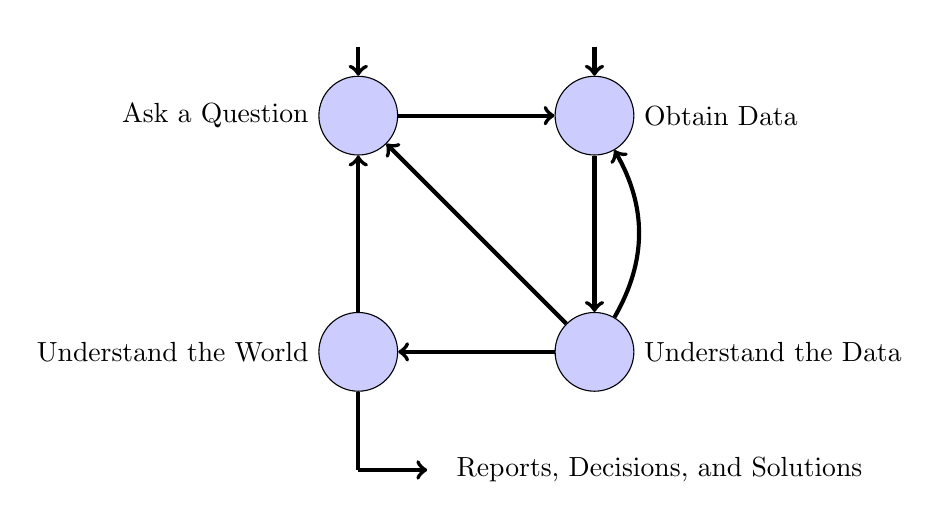
\begin{tikzpicture}
				\node[circle, draw, inner sep = 0pt, minimum width = 1cm, fill = blue!20] at (0,0) (understand_world) {};
				\node[circle, draw, inner sep = 0pt, minimum width = 1cm, fill = blue!20] at (0,3) (ask) {};s
				\node[circle, draw, inner sep = 0pt, minimum width = 1cm, fill = blue!20] at (3,3) (obtain) {};
				\node[circle, draw, inner sep = 0pt, minimum width = 1cm, fill = blue!20] at (3,0) (understand_data) {};
				
				\node at (0,4) (topask) {};
				\node at (3,4) (topobtain) {};
				
				\node at (0,-1.5) (ghostnode) {};
				\node at (1,-1.5) (report) {};
				
				\node[left] at (ask.west){Ask a Question};
				\node[left] at (understand_world.west){Understand the World};
				\node[right] at (obtain.east){Obtain Data};
				\node[right] at (understand_data.east){Understand the Data};
				\node[right] at (report.east){Reports, Decisions, and Solutions};
				
				\draw (understand_world) edge [->, line width = 1.5pt] (ask);
				\draw (understand_data) edge [->, line width = 1.5pt] (understand_world);
				\draw (understand_data) edge [->, line width = 1.5pt] (ask);
				\draw (ask) edge [->, line width = 1.5pt] (obtain);
				\draw (obtain) edge [->, line width = 1.5pt] (understand_data);
				\draw (understand_data) edge[bend right, ->, line width = 1.5pt] node [left] {} (obtain);
				
				\draw (topask) edge [->, line width = 1.5pt] (ask);
				\draw (topobtain) edge [->, line width = 1.5pt] (obtain);
				
				\draw (understand_world) edge [line width = 1.5pt] (ghostnode.center);
				\draw (ghostnode.center) edge [->, line width = 1.5pt] (report);
			\end{tikzpicture}
		
			\newframe
			% FRAME 2 %
			\begin{tikzpicture}
				\node[circle, draw, inner sep = 0pt, minimum width = 1cm, fill = blue!20, opacity = 0.25] at (0,0) (understand_world) {};
				\node[circle, draw, inner sep = 0pt, minimum width = 1cm, fill = blue!20] at (0,3) (ask) {};s
				\node[circle, draw, inner sep = 0pt, minimum width = 1cm, fill = blue!20, opacity = 0.25] at (3,3) (obtain) {};
				\node[circle, draw, inner sep = 0pt, minimum width = 1cm, fill = blue!20, opacity = 0.25] at (3,0) (understand_data) {};
				
				\node at (0,4) (topask) {};
				\node at (3,4) (topobtain) {};
				
				\node at (0,-1.5) (ghostnode) {};
				\node at (1,-1.5) (report) {};
				
				\node[left] at (ask.west){\color{darkblue}{\textbf{Ask a Question}}};
				\node[left, opacity = 0.25] at (understand_world.west){Understand the World};
				\node[right, opacity = 0.25] at (obtain.east){Obtain Data};
				\node[right, opacity = 0.25] at (understand_data.east){Understand the Data};
				\node[right, opacity = 0.25] at (report.east){Reports, Decisions, and Solutions};
				
				\draw (understand_world) edge [->, line width = 1.5pt] (ask);
				\draw (understand_data) edge [->, line width = 1.5pt, opacity = 0.25] (understand_world);
				\draw (understand_data) edge [->, line width = 1.5pt] (ask);
				\draw (ask) edge [->, line width = 1.5pt] (obtain);
				\draw (obtain) edge [->, line width = 1.5pt, opacity = 0.25] (understand_data);
				\draw (understand_data) edge[bend right, ->, line width = 1.5pt, opacity = 0.25] node [left] {} (obtain);
				
				\draw (topask) edge [->, line width = 1.5pt] (ask);
				\draw (topobtain) edge [->, line width = 1.5pt, opacity = 0.25] (obtain);
				
				\draw (understand_world) edge [line width = 1.5pt, opacity = 0.25] (ghostnode.center);
				\draw (ghostnode.center) edge [->, line width = 1.5pt, opacity = 0.25] (report);
			\end{tikzpicture}
		
			\newframe
			% FRAME 3 %
			\begin{tikzpicture}
				\node[circle, draw, inner sep = 0pt, minimum width = 1cm, fill = blue!20, opacity = 0.25] at (0,0) (understand_world) {};
				\node[circle, draw, inner sep = 0pt, minimum width = 1cm, fill = blue!20, opacity = 0.25] at (0,3) (ask) {};s
				\node[circle, draw, inner sep = 0pt, minimum width = 1cm, fill = blue!20] at (3,3) (obtain) {};
				\node[circle, draw, inner sep = 0pt, minimum width = 1cm, fill = blue!20, opacity = 0.25] at (3,0) (understand_data) {};
				
				\node at (0,4) (topask) {};
				\node at (3,4) (topobtain) {};
				
				\node at (0,-1.5) (ghostnode) {};
				\node at (1,-1.5) (report) {};
				
				\node[left, opacity = 0.25] at (ask.west){Ask a Question};
				\node[left, opacity = 0.25] at (understand_world.west){Understand the World};
				\node[right] at (obtain.east){\color{darkblue}{\textbf{Obtain Data}}};
				\node[right, opacity = 0.25] at (understand_data.east){Understand the Data};
				\node[right, opacity = 0.25] at (report.east){Reports, Decisions, and Solutions};
				
				\draw (understand_world) edge [->, line width = 1.5pt, opacity = 0.25] (ask);
				\draw (understand_data) edge [->, line width = 1.5pt, opacity = 0.25] (understand_world);
				\draw (understand_data) edge [->, line width = 1.5pt, opacity = 0.25] (ask);
				\draw (ask) edge [->, line width = 1.5pt] (obtain);
				\draw (obtain) edge [->, line width = 1.5pt] (understand_data);
				\draw (understand_data) edge[bend right, ->, line width = 1.5pt] node [left] {} (obtain);
				
				\draw (topask) edge [->, line width = 1.5pt, opacity = 0.25] (ask);
				\draw (topobtain) edge [->, line width = 1.5pt] (obtain);
				
				\draw (understand_world) edge [line width = 1.5pt, opacity = 0.25] (ghostnode.center);
				\draw (ghostnode.center) edge [->, line width = 1.5pt, opacity = 0.25] (report);
			\end{tikzpicture}
		
			\newframe
			% FRAME 4 %
			\begin{tikzpicture}
				\node[circle, draw, inner sep = 0pt, minimum width = 1cm, fill = blue!20, opacity = 0.25] at (0,0) (understand_world) {};
				\node[circle, draw, inner sep = 0pt, minimum width = 1cm, fill = blue!20, opacity = 0.25] at (0,3) (ask) {};s
				\node[circle, draw, inner sep = 0pt, minimum width = 1cm, fill = blue!20, opacity = 0.25] at (3,3) (obtain) {};
				\node[circle, draw, inner sep = 0pt, minimum width = 1cm, fill = blue!20] at (3,0) (understand_data) {};
				
				\node at (0,4) (topask) {};
				\node at (3,4) (topobtain) {};
				
				\node at (0,-1.5) (ghostnode) {};
				\node at (1,-1.5) (report) {};
				
				\node[left, opacity = 0.25] at (ask.west){Ask a Question};
				\node[left, opacity = 0.25] at (understand_world.west){Understand the World};
				\node[right, opacity = 0.25] at (obtain.east){Obtain Data};
				\node[right] at (understand_data.east){\color{darkblue}{\textbf{Understand the Data}}};
				\node[right, opacity = 0.25] at (report.east){Reports, Decisions, and Solutions};
				
				\draw (understand_world) edge [->, line width = 1.5pt, opacity = 0.25] (ask);
				\draw (understand_data) edge [->, line width = 1.5pt] (understand_world);
				\draw (understand_data) edge [->, line width = 1.5pt] (ask);
				\draw (ask) edge [->, line width = 1.5pt, opacity = 0.25] (obtain);
				\draw (obtain) edge [->, line width = 1.5pt] (understand_data);
				\draw (understand_data) edge[bend right, ->, line width = 1.5pt] node [left] {} (obtain);
				
				\draw (topask) edge [->, line width = 1.5pt, opacity = 0.25] (ask);
				\draw (topobtain) edge [->, line width = 1.5pt, opacity = 0.25] (obtain);
				
				\draw (understand_world) edge [line width = 1.5pt, opacity = 0.25] (ghostnode.center);
				\draw (ghostnode.center) edge [->, line width = 1.5pt, opacity = 0.25] (report);
			\end{tikzpicture}
		
			\newframe
			% FRAME 5 %
			\begin{tikzpicture}
				\node[circle, draw, inner sep = 0pt, minimum width = 1cm, fill = blue!20] at (0,0) (understand_world) {};
				\node[circle, draw, inner sep = 0pt, minimum width = 1cm, fill = blue!20, opacity = 0.25] at (0,3) (ask) {};s
				\node[circle, draw, inner sep = 0pt, minimum width = 1cm, fill = blue!20, opacity = 0.25] at (3,3) (obtain) {};
				\node[circle, draw, inner sep = 0pt, minimum width = 1cm, fill = blue!20, opacity = 0.25] at (3,0) (understand_data) {};
				
				\node at (0,4) (topask) {};
				\node at (3,4) (topobtain) {};
				
				\node at (0,-1.5) (ghostnode) {};
				\node at (1,-1.5) (report) {};
				
				\node[left, opacity = 0.25] at (ask.west){Ask a Question};
				\node[left] at (understand_world.west){\color{darkblue}{\textbf{Understand the World}}};
				\node[right, opacity = 0.25] at (obtain.east){Obtain Data};
				\node[right, opacity = 0.25] at (understand_data.east){Understand the Data};
				\node[right] at (report.east){Reports, Decisions, and Solutions};
				
				\draw (understand_world) edge [->, line width = 1.5pt] (ask);
				\draw (understand_data) edge [->, line width = 1.5pt] (understand_world);
				\draw (understand_data) edge [->, line width = 1.5pt, opacity = 0.25] (ask);
				\draw (ask) edge [->, line width = 1.5pt, opacity = 0.25] (obtain);
				\draw (obtain) edge [->, line width = 1.5pt, opacity = 0.25] (understand_data);
				\draw (understand_data) edge[bend right, ->, line width = 1.5pt, opacity = 0.25] node [left] {} (obtain);
				
				\draw (topask) edge [->, line width = 1.5pt, opacity = 0.25] (ask);
				\draw (topobtain) edge [->, line width = 1.5pt, opacity = 0.25] (obtain);
				
				\draw (understand_world) edge [line width = 1.5pt] (ghostnode.center);
				\draw (ghostnode.center) edge [->, line width = 1.5pt] (report);
			\end{tikzpicture}
		}
	\end{animateinline}
\end{center}

The Data Science Lifecycle goes as follows:
\begin{enumerate}
	\item \textbf{Question/Problem Formulation}
	\begin{itemize}
		\item What do we want to know?
		\item What problems are we trying to solve?
		\item What hypotheses do we want to test?
		\item What are our metrics for success?
	\end{itemize}
	\item \textbf{Data Acquisition and Cleaning}
	\begin{itemize}
		\item What data do we have and what data do we need?
		\item How will we sample more data?
		\item Is our data representative of the population we want to study?
	\end{itemize}
	\item \textbf{Exploratory Data Analysis and Visualization}
	\begin{itemize}
		\item How is our data organized, and what does it contain?
		\item Do we already have the relevant data?
		\item What are the biases, anomalies, or other issues with the data?
		\item How do we transform the data to enable effective analysis?
	\end{itemize}
	\item \textbf{Prediction and Inference}
	\begin{itemize}
		\item What does the data say about the world?
		\item Does it answer our questions or accurately solve the problem?
		\item How robust are our conclusions and can we trust the predictions?
	\end{itemize}
\end{enumerate}
\end{document}